In this chapter, we explore the experimental design, results, and discussion of the study, focusing on the frequency distribution and sentiment analysis of Reddit comments related to climate change. The data source is "The Reddit Climate Change Dataset" which provides a comprehensive collection of comments from Reddit covering the years 2010 to 2022. We will explore how the volume of discussions and their sentiment have evolved over time, providing insights into public discourse on climate change.

\section{Frequency of Reddit Comments}
The first image (Figure \ref{fig:all_samples}) displays the absolute frequency of Reddit comments per year from 2010 to 2022. It is evident from the graph that there is a significant increase in the volume of comments over the years. Starting from a modest count in 2010, there is a sharp rise in 2019, peaking at 978,413 comments. This increase can be attributed to increased global awareness and discussions around climate change, fueled by significant events such as the Fridays for Future movement \cite{context2024greta,greenhouse2024greta} and the Australian bushfires \cite{wwf2024bushfires}. The years following 2019 show a slight decrease but remain significantly higher than the initial years. On average, the number of comments per year is 162,258 for Negative, 32,573 for Neutral, and 159,068 for Positive sentiments. The standard deviation for these classes is 151,771 for Negative, 31,635 for Neutral, and 143,654 for Positive sentiments, indicating considerable variability in the annual comment frequencies.
\begin{figure}[h]    
    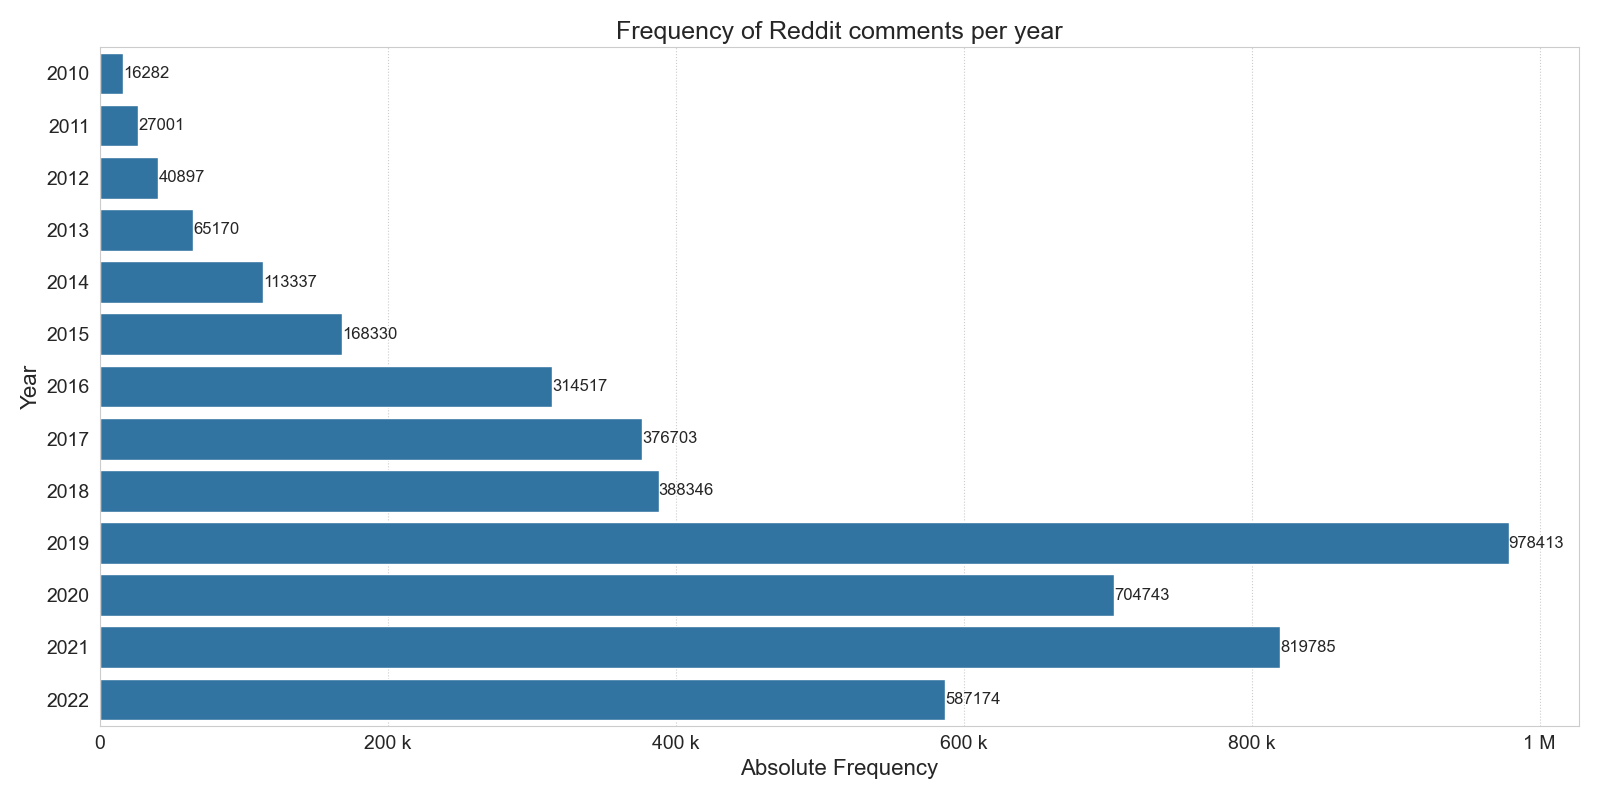
\includegraphics[width=\textwidth]{images/overview/samples_all.png}
    \caption{Distribution of Comments on Climate Change per Year}
    \label{fig:all_samples}
\end{figure}
This trend reflects the growing interest and concern among the public regarding climate change. The increase in comment frequency can be linked to major global events that brought climate issues to the forefront of public discourse. For example, the year 2019 saw a notable increase in comments, which coincides with widespread climate protests and significant media coverage of environmental issues \cite{euronews2023greta}.
The following image (Figure \ref{fig:all_samples_by_class}) breaks down these frequencies by sentiment class—positive, neutral, and negative—providing a more detailed view. Each bar is divided into three segments representing the proportion of each sentiment class. While the total volume of negative comments is higher overall, negative sentiment comments exceed positive ones in only four years: 2018, 2019, 2020, and 2022. This indicates that during these specific years, there were more discussions with a negative sentiment towards climate change topics among Reddit users. This could reflect increased awareness and concern about climate change impacts during those years, driven by specific events or developments. The year 2019 stands out with the highest number of negative comments, reflecting the heightened anxiety and negative sentiment during that period.
The dominance of negative sentiments suggests that climate change discussions on Reddit are often driven by worries and negative perceptions. This could be due to the alarming nature of news related to climate change, such as reports on natural disasters, policy failures, and scientific warnings about the impacts of climate change \cite{earthday2023climate}.
\begin{figure}[h]
    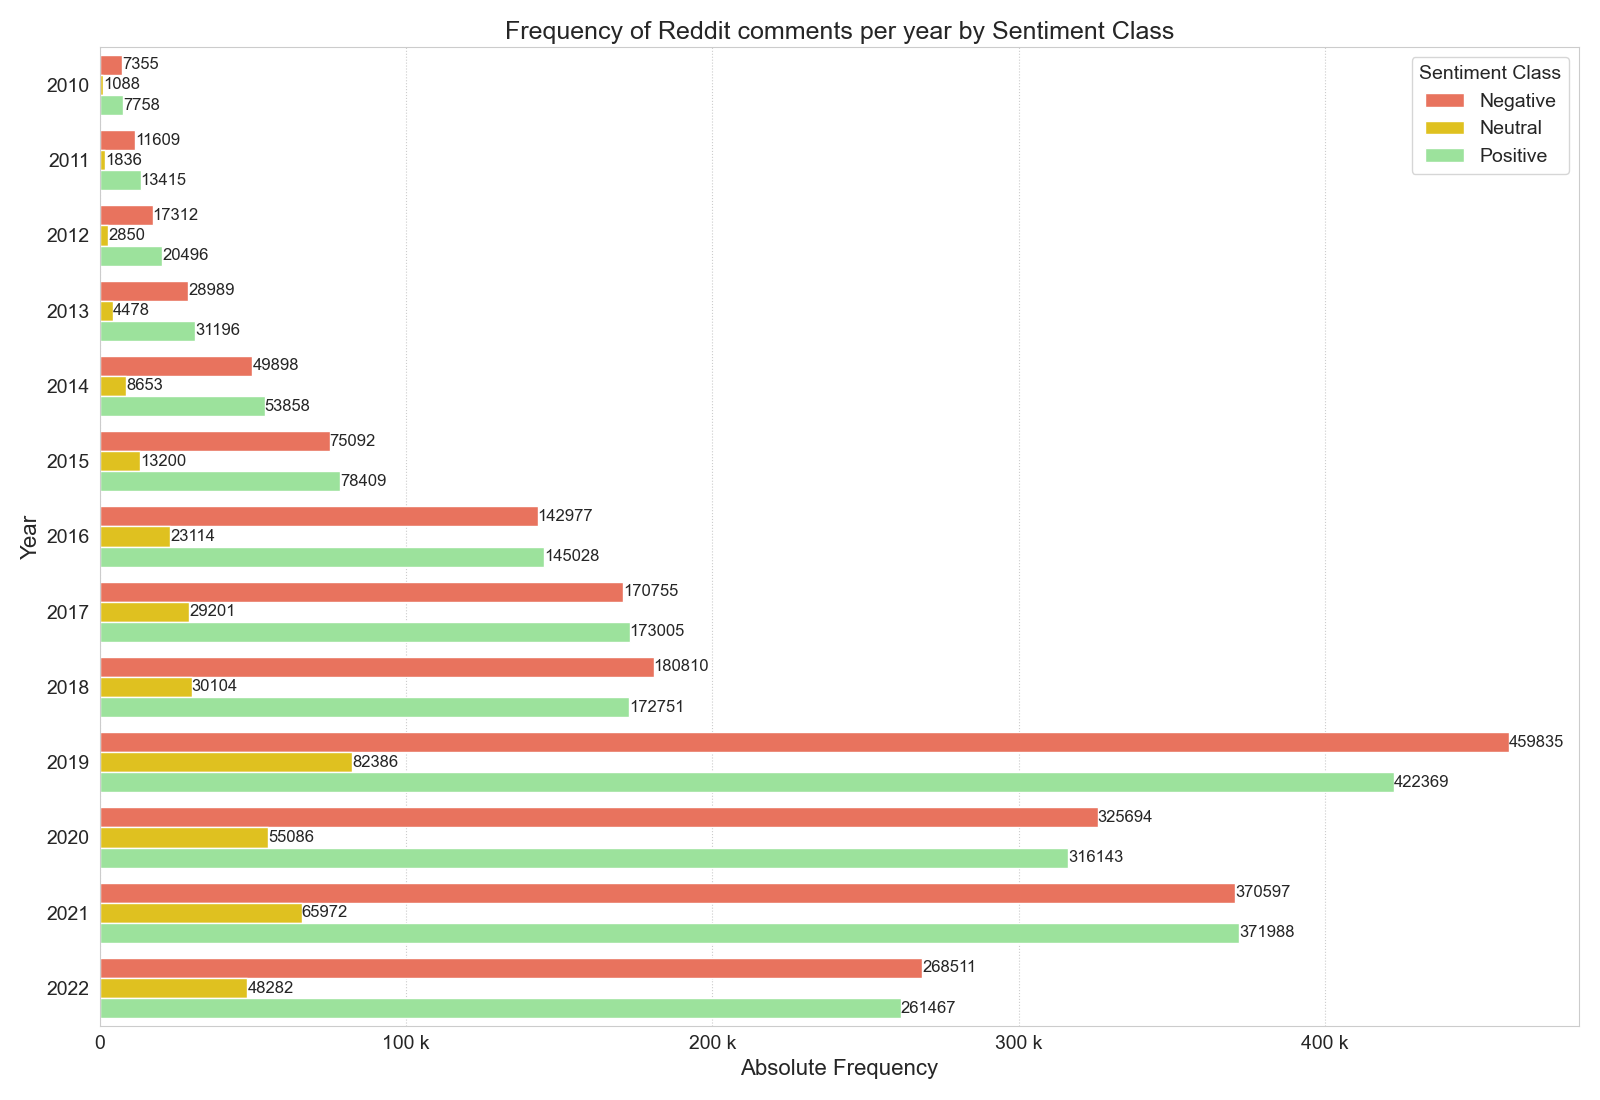
\includegraphics[width=\textwidth]{images/overview/samples_all_by_class.png}
    \caption{Distribution of Samples per Year by Sentiment Class}
    \label{fig:all_samples_by_class}
\end{figure}

\section{Distribution of Sentiment Classes}
\begin{figure}[h!]
    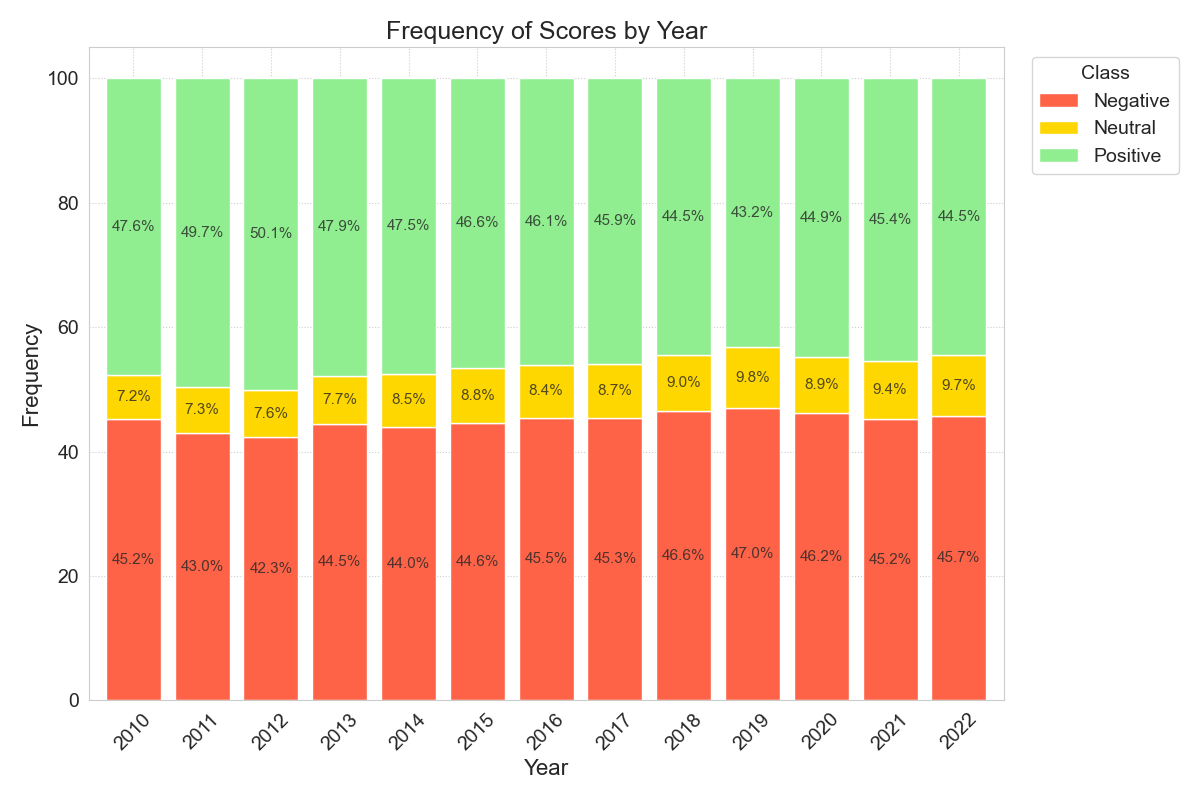
\includegraphics[width=\textwidth]{images/overview/samples_all_by_class_stacked.png}
    \caption{Percentage Distribution of Comments on Climate Change per Year by Sentiment Class}
    \label{fig:all_samples_by_class_percentage}
\end{figure}
In Figure \ref{fig:all_samples_by_class_percentage}, the percentage distribution of sentiment classes per year is presented. This stacked bar chart shows that while negative sentiments dominate the years 2018-2020 and 2022, there is a noticeable portion of positive and neutral sentiments as well. The proportion of neutral comments remains relatively stable, while positive comments show slight variations. The increase in negative sentiments around 2019 correlates with significant climate-related events that year, as previously mentioned. The data indicates that the public discourse on Reddit tends to be more critical or concerned regarding climate change.
Displaying both absolute numbers (Figure \ref{fig:all_samples_by_class}) and relative values (Figure \ref{fig:all_samples_by_class_percentage}) in sentiment analysis plots provides a comprehensive view of the data. The absolute numbers reveal the overall volume of comments, indicating trends in user engagement, while the relative values show the proportion of each sentiment class, highlighting shifts in sentiment distribution over time. This dual approach ensures a more detailed understanding of sentiment trends.
The persistent presence of negative sentiments highlights a continuous public concern about climate change. Neutral comments, which make up a considerable portion, likely include factual statements and information sharing, indicating that many users are discussing climate change in an informative manner. The slight variations in positive comments suggest occasional optimism, possibly related to breakthroughs in climate science, successful environmental policies, or inspiring activism.

\section{Mean Sentiment Over Time}
The image in Figure \ref{fig:mean_sentiment} plots the mean VADER sentiment score per year, providing an overview of the general sentiment trend. The sentiment scores fluctuate over the years, with notable peaks and drops corresponding to significant climate-related events. For instance, the negative decrease around 2018 aligns with the intense climate protests and global movements that provoked widespread discussions and emotional responses. Overall, the sentiment trend illustrates the evolving public sentiment towards climate change, marked by periods of optimism and concern.
The mean sentiment score reveals the general mood of the public regarding climate change over time. The positive peaks might correlate with successful climate initiatives or positive media coverage, while the negative drops reflect times of crisis or heightened awareness of climate issues. This trend underscores the impact of global events and media coverage on public sentiment, highlighting the dynamic nature of climate change discourse on social media \cite{Valentini2016}.

A significant factor influencing these discussions is the role of influential climate activists such as Greta Thunberg. Greta Thunberg, a Swedish environmental activist, gained international recognition for her efforts to tackle climate change. Her Fridays for Future movement, which began as a solo protest outside the Swedish parliament, inspired millions of young people around the world to participate in climate strikes \cite{fridaysforfuture2024ruckblick}. Thunberg's speeches at major international forums, including the United Nations \cite{un2019greta}, have inspired public opinion and brought the urgency of climate action to the forefront of global discourse (Jones, 2021).
Thunberg's activism, particularly around 2018 and 2019, contributed to the surge in climate-related discussions on Reddit. Her ability to express the fears and hopes of a younger generation has had a significant impact on many, driving both positive and negative sentiments in online discussions. The increase in negative sentiments during these years can be partly attributed to the polarized reactions to her outspoken stance on climate issues \cite{aidr2024blacksummer}.

This detailed examination provides a comprehensive overview of the dynamics of climate change discourse on Reddit, highlighting the patterns of public sentiment and the influence of significant global events and prominent activists. The data underscores the complex interplay between public opinion, media coverage, and impactful events in shaping the conversation around climate change.

\begin{figure}    
    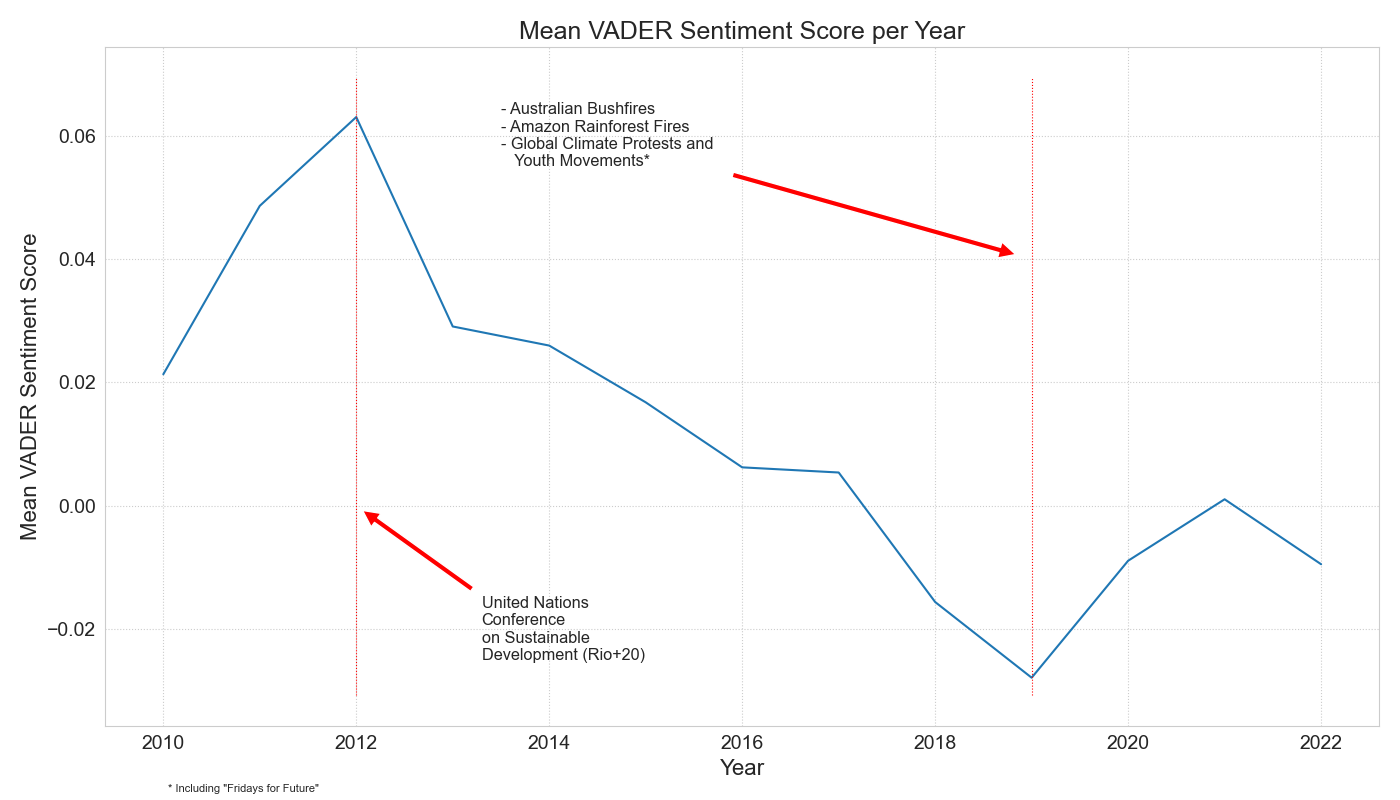
\includegraphics[width=\textwidth]{images/overview/mean_sentiment.png}
    \caption{Annual Average Sentiment with Event Highlighting}
    \label{fig:mean_sentiment}
\end{figure}

\section{Top 5 Frequent Subreddits}
\begin{figure}
    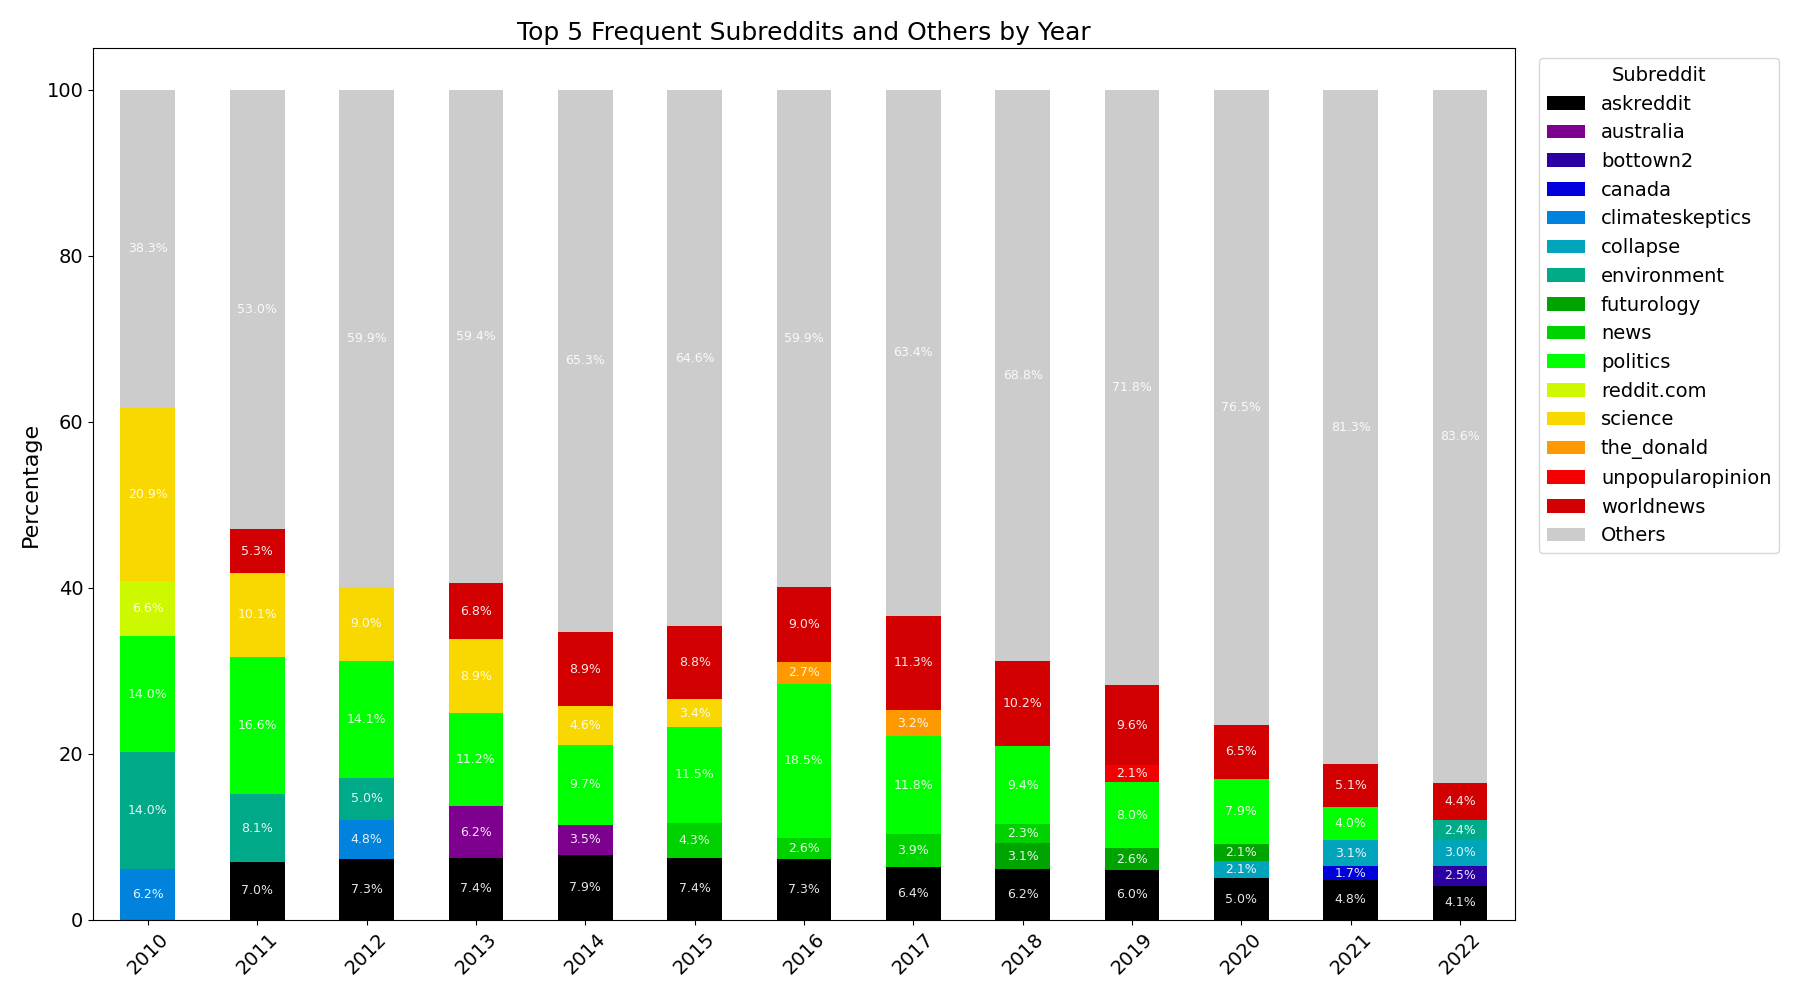
\includegraphics[width=\textwidth]{images/overview/subreddit_frequency_top5.png}
    \caption{Yearly Top Five Subreddits and their Percentual Relation}
    \label{fig:top5subreddits}
\end{figure}
Figure \ref{fig:top5subreddits} illustrates the five most frequent subreddits by year, alongside a category labeled \emph{Others}. This graph provides insight into which subreddits are most active in discussions about climate change. The \emph{Others} category covers all subreddits that are not within the top five for a given year, highlighting the contributions of a broad range of subreddits to the climate change discourse. The dominance of \emph{Others} suggests that climate change is a topic of widespread interest across many different communities on Reddit, indicating that it becomes more relevant to more areas of our life and conversations. Specific subreddits such as \emph{worldnews}, \emph{science}, and \emph{politics} are consistently among the top contributors, reflecting the intersection of climate change with global events, scientific discussion, and political debate.

The diverse range of subreddits involved in climate change discussions, as indicated by the significant \emph{Others} category, suggests that the topic spreads through various aspects of society, from politics and science to general news and public opinion \cite{doi:10.1177/1329878X211038004}. The presence of subreddits like \emph{the\_donald} and \emph{unpopularopinion} in certain years indicates that climate change is also a point of debate and differing viewpoints. The fluctuation in subreddit participation over the years can reflect shifts in public interest and the emergence of new influential communities on Reddit.

\section{Comment Length Analysis}
\begin{figure}[h]
    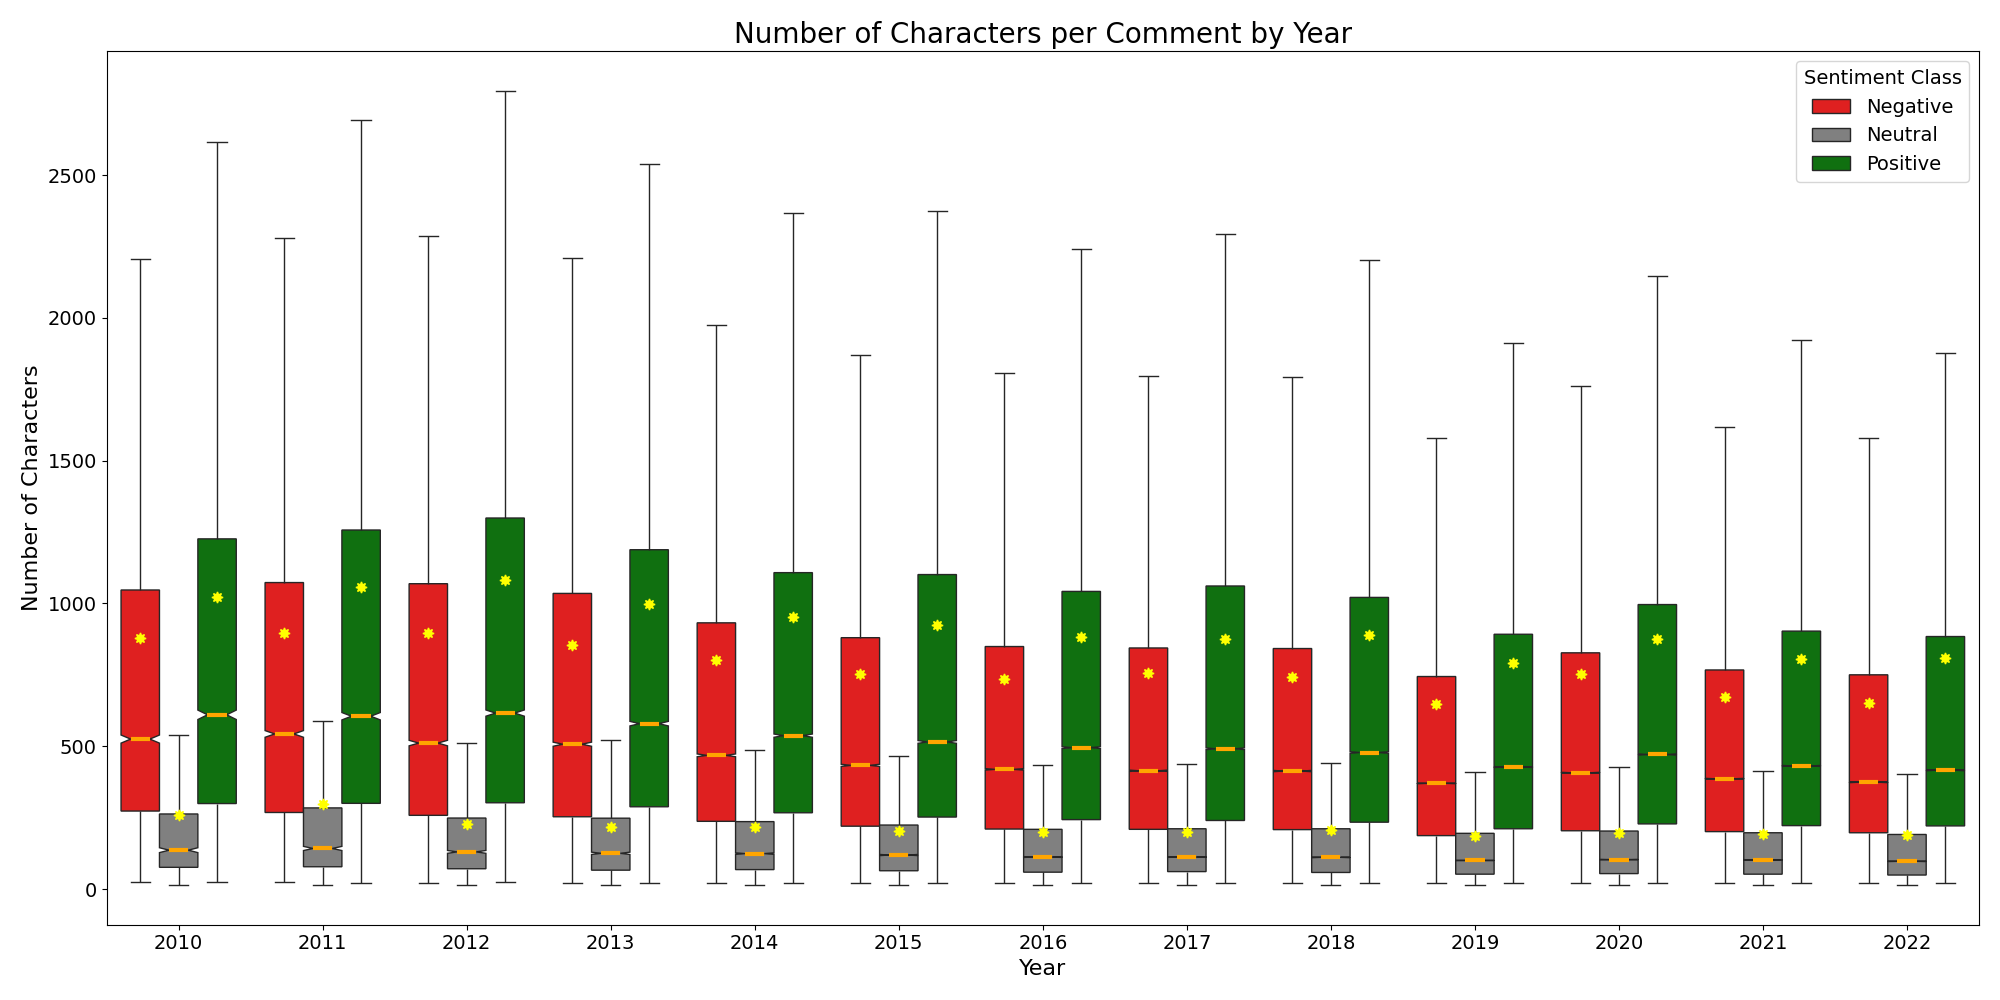
\includegraphics[width=\textwidth]{images/overview/comment_length_boxplot.png}
    \caption{Boxplot of the Comment Length by Sentiment Class}
    \label{fig:boxplot_comment_length}
\end{figure}
Figure \ref{fig:boxplot_comment_length} displays a boxplot of the number of characters per comment by year, segmented by sentiment class. This analysis reveals that comments with positive sentiments tend to be longer compared to those with negative or neutral sentiments. The longer length of positive comments indicates that these discussions are often more detailed and elaborate. On average, the length of negative comments is 706.76 characters with a standard deviation of 984.78, neutral comments average 195.46 characters with a standard deviation of 382.73, and positive comments average 848.30 characters with a standard deviation of 1177.78. This indicates a considerable variability in comment lengths, particularly for positive comments.
Longer comments usually show more detailed discussions. The data shows that users tend to write more extensively when expressing positive sentiments, possibly to share their support for climate initiatives or detailed success stories. These positive comments help build a supportive environment and promote constructive discussions about climate change solutions. Negative comments, while generally shorter, might still reflect strong emotions such as frustration or anger, leading users to provide critiques or express their feelings. Neutral comments are typically the shortest, focusing on sharing straightforward information without much additional commentary \cite{orglearning}.
Understanding these patterns is important for several reasons. First, the depth of engagement in positive comments suggests that users who are optimistic about climate change solutions are more likely to share detailed information and experiences. This can enrich the conversation and provide valuable insights for others. Recognizing the potential for detailed negative comments driven by frustration can help ensure that these contributions remain constructive and do not escalate tensions.

In conclusion, this confirms that positive comments on climate change tend to be more detailed and longer compared to negative and neutral comments. This trend is constant across all the years analyzed, indicating that positive discussions involve more complex and extensive commentary. Understanding these patterns is crucial for promoting meaningful conversations about climate change and ensuring a balanced discourse that includes both emotional and factual content.